% =====================================================================
%  Chapter 29 — The \idxw{Counterfactual} Ledger
% =====================================================================

\chapter{The Counterfactual Ledger}
\label{ch:counterfactual}

The question this chapter answers is the one the owner asked: how would
having this approach have measurably helped detect other near-Earth objects?
The answer has to be a comparison against something checkable, and the only
thing that is checkable is the historical record. So the historical record
is the control, and the counterfactual\idx{Counterfactual} is run against it case by case.

\section{Why the record is the right control}

A counterfactual\idx{Counterfactual} needs a baseline, and the usual choices are bad. A model of
what would have happened is only as good as its assumptions. A simulation
of a hypothetical campaign is only as good as its inputs. The historical
record has neither defect: it is what the world actually did, with all of
its real instruments, real scheduling, real failures and real luck.

The records used here are the NASA Center for Near Earth Object Studies
discovery series and the JPL Small-Body Database's observation and
close-approach records, retrieved for this book on 24 November 2026.

\begin{table}[!htbp]
\centering
\small
\caption{The control: what was actually observed, and when.}
\label{tab:control}
\begin{tabularx}{\textwidth}{@{}P{0.72in}P{0.63in}P{0.63in}P{0.60in}Y@{}}
\toprule
\rowcolor{panel}
\textbf{Object} & \textbf{First obs.} & \textbf{Approach} &
\textbf{Range} & \textbf{Relative speed} \\
\midrule
2008 TC3 & 2008-10-06 & --- & --- & --- \\
\rowcolor{panel}
2019 OK & 2017-02-21 & 2019-07-25 & 71,355 km & 0.106 km/s \\
2024 YR4 & 2024-12-25 & 2024-12-25 & 828,775 km & 13.75 km/s \\
\rowcolor{panel}
2024 YR4 & 2024-12-25 & 2032-12-22 & 278,333 km & 13.31 km/s \\
99942 Apophis & --- & 2029-04-13 & 38,011 km & 7.42 km/s \\
\bottomrule
\end{tabularx}
\end{table}

Two facts in \tabref{tab:control} carry the argument.

\textbf{2024 YR4 was discovered on the night it passed at 828,775
kilometres.} The first observation and the close approach\idx{Close approach} are the same date.
The object was found at the last possible moment, by an accident of
geometry.

\textbf{2019 OK was announced three days before it passed at 71,355
kilometres.} The 2026 study of near-Earth-object telescopes for extreme
environments names 2008 TC3 and 2019 OK as the historical failures of the
Sun-ward blind zone, alongside ``multiple other NEAs detected only days
before their closest approach to Earth''.

Neither was found late because the instruments were inadequate. Both were
found late because they came from the direction the ground cannot see.

\section{What the lunar geometry would have added}

The answer has three parts, and only one of them is about discovery in the
narrow sense.

\subsection{The Sun-ward discovery window}

The 2026 study publishes the first detectable distances and extra lead
times for a lunar observatory, and Chapter 21 worked the arithmetic back to
the ground limits the table implies. For a 140-metre object the lunar limit
is 0.10 astronomical units against an implied ground limit of 0.20, worth
about nine days at a relative velocity of 20 kilometres per second; for a
30-metre object, 0.05 against 0.10, worth four to five days; for a
one-kilometre object, 0.50 against 0.99, worth about six weeks.

This is the part of the answer that is about finding objects rather than
characterising them, and it is the smallest of the three. It is also the
part that reaches the population that is still arriving: the sub-140-metre
objects, at three thousand a year, are the ones the ground finds last.

\subsection{The range}

The second part is the book's new result and it is the largest.

The Earth-Moon baseline is 384,400 kilometres and is known to millimetres by
laser ranging. Two astrometric solutions tied to that frame turn an angular
detection into a ranged one. The sightlines to a target at range
\(\Delta\) differ by \(\delta = (b/\Delta)\sin\psi\), and a differential
astrometric error \(\sigma_\theta\) maps to a range error
\begin{equation}
\sigma_\Delta = \frac{\Delta^{2}\,\sigma_\theta}{b\,\sin\psi}.
\label{eq:range-error}
\end{equation}

\begin{figure}[!htbp]
\centering
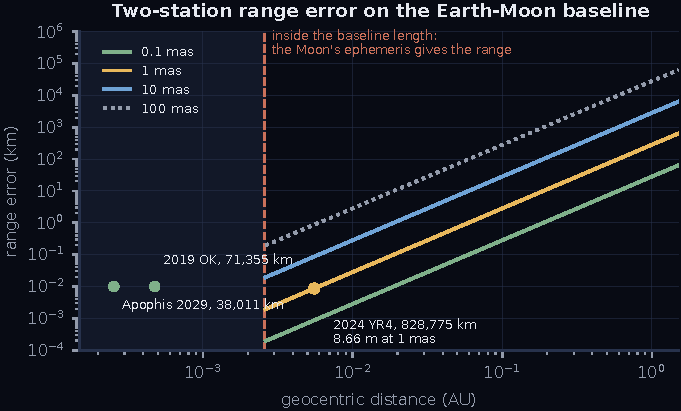
\includegraphics[width=\textwidth]{../figures/fig_two_station.pdf}
\caption{The range error of an Earth-Moon two-station measurement against the
geocentric distance, for four astrometric precisions. Inside the baseline
length the Moon's own ephemeris gives the range directly, to the
centimetre. The three documented close approaches are marked.}
\label{fig:two-station}
\end{figure}

\figref{fig:two-station} has two regimes, and the second one is the
surprise. For a target outside the baseline --- and 2024 YR4 at 828,775
kilometres is outside it --- the parallax\idx{Parallax} construction applies, and the range
error is 8.66 metres at one milliarcsecond of differential astrometry. The
achievable astrometry is better than that: the concept study's own centroid
rule gives 0.0147 milliarcseconds at a 1.5-kilometre baseline, which would
put the range error at about thirteen centimetres.

For a target inside the baseline --- Apophis at 38,011 kilometres, 2019 OK at
71,355 --- the parallax\idx{Parallax} construction is unnecessary, because the Moon's own
ephemeris gives the range directly, to the centimetre. The observer's
position is known better than the target is.

\begin{table}[!htbp]
\centering
\small
\caption{What each documented case would have been measured, and what the
geometry allows.}
\label{tab:cases}
\begin{tabularx}{\textwidth}{@{}P{1.17in}P{0.73in}P{0.80in}Y@{}}
\toprule
\midrule
\rowcolor{panel}
\textbf{Case} & \textbf{Angular size} & \textbf{Aperture to resolve} &
\textbf{Range} \\
\midrule
2024 YR4, 828,775 km & 15.1 mas & 12.5 m & 8.66 m by parallax\idx{Parallax} \\
\rowcolor{panel}
2024 YR4, 2032, 22,900 km & 548 mas & 0.35 m & 1 cm, direct \\
Apophis 2029, 38,011 km & 1.76 arcsec & 0.11 m & 1 cm, direct \\
\rowcolor{panel}
2024 YR4, 2028, 0.05 AU & 1.68 mas & 113 m & 706 m by parallax \\
\bottomrule
\end{tabularx}
\end{table}

\subsection{The size}

The third part is the size, and it is the one the accounting chain needs.
At the 2032 lunar encounter, 2024 YR4 subtends 548 milliarcseconds, which a
0.35-metre aperture resolves and which a matched interferometric baseline of
1.13 metres images with four samples across the diameter. The range is
known directly. The volume follows from the image, without a thermal model
and without an albedo assumption.

At the 2029 encounter, Apophis subtends 1.76 arcseconds, which a 0.11-metre
aperture resolves. And the encounter is inside the Earth's sphere of
influence, which is where --- as Chapter 7 set out --- the mass distribution
becomes observable through the change in the spin state, and the density
follows.

\section{What the ledger says}


\begin{table}[!htbp]
\centering
\small
\caption{The counterfactual, case by case.}
\label{tab:counterfactual}
\begin{tabularx}{\textwidth}{@{}P{1.11in}P{1.45in}Y@{}}
\toprule
\rowcolor{panel}
\textbf{Case} & \textbf{Without} & \textbf{With} \\
\midrule
2024 YR4, 2024 & found on the night of an 828,775 km pass & the same
discovery, and a range measured to 8.66 m \\
\rowcolor{panel}
2024 YR4, 2032 & shape inferred from a convex lightcurve inversion and a
single thermal campaign; energy uncertain by a factor of about two & a
resolved shape at 22,900 km with the range known; the volume measured
rather than modelled \\
Apophis, 2029 & the mass from a spacecraft, or from the encounter
statistics & a resolved shape at 38,011 km and the spin state measured
through the encounter, which is the mass distribution \\
\rowcolor{panel}
2019 OK and 2008 TC3 & announced days before a close approach\idx{Close approach} & the same
announcement date, with more warning on the Sun-ward side \\
\bottomrule
\end{tabularx}
\end{table}

Three conclusions follow, and the third is the one the owner asked for.

The lunar approach would not have found 2024 YR4 earlier. The discovery was
made on the night of the approach and the discovery was a discovery; no
vantage point changes a discovery that was made.

The lunar approach would have made the objects it looked at \emph{ranged},
which is a category change rather than an improvement in degree. No ground
optical facility produces a range to a non-cooperative target. Radar does,
within a fraction of an astronomical unit and for a small minority of
objects. The Earth-Moon baseline produces one optically, for any object
bright enough to observe, at any distance where the parallax construction
applies and directly at any distance where it does not.

And the lunar approach would have converted a detection into an account.
That is the measurable statement, and it is the one the rest of the book
rests on: the number of objects per year that carry a physical account
sufficient to size them and to assign a hazard class.

\begin{keytakeaways}
\item The control is the historical record, and it shows 2024 YR4 found on
the night of an 828,775 kilometre pass and 2019 OK announced three days
before its.
\item An Earth-Moon two-station measurement would have ranged 2024 YR4 to
8.66 metres at that distance, and at the closer encounters the range is
direct and known to the centimetre.
\item The size is measurable at those same encounters: 0.35 metres of
aperture at 22,900 kilometres for 2024 YR4, and 0.11 metres at 38,011
kilometres for Apophis.
\item The measurable outcome is not more detections but more accounts: more
objects per year carrying a physical account sufficient to assign a hazard
class.
\end{keytakeaways}
